\documentclass[1p]{elsarticle_modified}
%\bibliographystyle{elsarticle-num}

%\usepackage[colorlinks]{hyperref}
%\usepackage{abbrmath_seonhwa} %\Abb, \Ascr, \Acal ,\Abf, \Afrak
\usepackage{amsfonts}
\usepackage{amssymb}
\usepackage{amsmath}
\usepackage{amsthm}
\usepackage{scalefnt}
\usepackage{amsbsy}
\usepackage{kotex}
\usepackage{caption}
\usepackage{subfig}
\usepackage{color}
\usepackage{graphicx}
\usepackage{xcolor} %% white, black, red, green, blue, cyan, magenta, yellow
\usepackage{float}
\usepackage{setspace}
\usepackage{hyperref}

\usepackage{tikz}
\usetikzlibrary{arrows}

\usepackage{multirow}
\usepackage{array} % fixed length table
\usepackage{hhline}

%%%%%%%%%%%%%%%%%%%%%
\makeatletter
\renewcommand*\env@matrix[1][\arraystretch]{%
	\edef\arraystretch{#1}%
	\hskip -\arraycolsep
	\let\@ifnextchar\new@ifnextchar
	\array{*\c@MaxMatrixCols c}}
\makeatother %https://tex.stackexchange.com/questions/14071/how-can-i-increase-the-line-spacing-in-a-matrix
%%%%%%%%%%%%%%%

\usepackage[normalem]{ulem}

\newcommand{\msout}[1]{\ifmmode\text{\sout{\ensuremath{#1}}}\else\sout{#1}\fi}
%SOURCE: \msout is \stkout macro in https://tex.stackexchange.com/questions/20609/strikeout-in-math-mode

\newcommand{\cancel}[1]{
	\ifmmode
	{\color{red}\msout{#1}}
	\else
	{\color{red}\sout{#1}}
	\fi
}

\newcommand{\add}[1]{
	{\color{blue}\uwave{#1}}
}

\newcommand{\replace}[2]{
	\ifmmode
	{\color{red}\msout{#1}}{\color{blue}\uwave{#2}}
	\else
	{\color{red}\sout{#1}}{\color{blue}\uwave{#2}}
	\fi
}

\newcommand{\Sol}{\mathcal{S}} %segment
\newcommand{\D}{D} %diagram
\newcommand{\A}{\mathcal{A}} %arc


%%%%%%%%%%%%%%%%%%%%%%%%%%%%%5 test

\def\sl{\operatorname{\textup{SL}}(2,\Cbb)}
\def\psl{\operatorname{\textup{PSL}}(2,\Cbb)}
\def\quan{\mkern 1mu \triangleright \mkern 1mu}

\theoremstyle{definition}
\newtheorem{thm}{Theorem}[section]
\newtheorem{prop}[thm]{Proposition}
\newtheorem{lem}[thm]{Lemma}
\newtheorem{ques}[thm]{Question}
\newtheorem{cor}[thm]{Corollary}
\newtheorem{defn}[thm]{Definition}
\newtheorem{exam}[thm]{Example}
\newtheorem{rmk}[thm]{Remark}
\newtheorem{alg}[thm]{Algorithm}

\newcommand{\I}{\sqrt{-1}}
\begin{document}

%\begin{frontmatter}
%
%\title{Boundary parabolic representations of knots up to 8 crossings}
%
%%% Group authors per affiliation:
%\author{Yunhi Cho} 
%\address{Department of Mathematics, University of Seoul, Seoul, Korea}
%\ead{yhcho@uos.ac.kr}
%
%
%\author{Seonhwa Kim} %\fnref{s_kim}}
%\address{Center for Geometry and Physics, Institute for Basic Science, Pohang, 37673, Korea}
%\ead{ryeona17@ibs.re.kr}
%
%\author{Hyuk Kim}
%\address{Department of Mathematical Sciences, Seoul National University, Seoul 08826, Korea}
%\ead{hyukkim@snu.ac.kr}
%
%\author{Seokbeom Yoon}
%\address{Department of Mathematical Sciences, Seoul National University, Seoul, 08826,  Korea}
%\ead{sbyoon15@snu.ac.kr}
%
%\begin{abstract}
%We find all boundary parabolic representation of knots up to 8 crossings.
%
%\end{abstract}
%\begin{keyword}
%    \MSC[2010] 57M25 
%\end{keyword}
%
%\end{frontmatter}

%\linenumbers
%\tableofcontents
%
\newcommand\colored[1]{\textcolor{white}{\rule[-0.35ex]{0.8em}{1.4ex}}\kern-0.8em\color{red} #1}%
%\newcommand\colored[1]{\textcolor{white}{ #1}\kern-2.17ex	\textcolor{white}{ #1}\kern-1.81ex	\textcolor{white}{ #1}\kern-2.15ex\color{red}#1	}

{\Large $\underline{12n_{0232}~(K12n_{0232})}$}

\setlength{\tabcolsep}{10pt}
\renewcommand{\arraystretch}{1.6}
\vspace{1cm}\begin{tabular}{m{100pt}>{\centering\arraybackslash}m{274pt}}
\multirow{5}{120pt}{
	\centering
	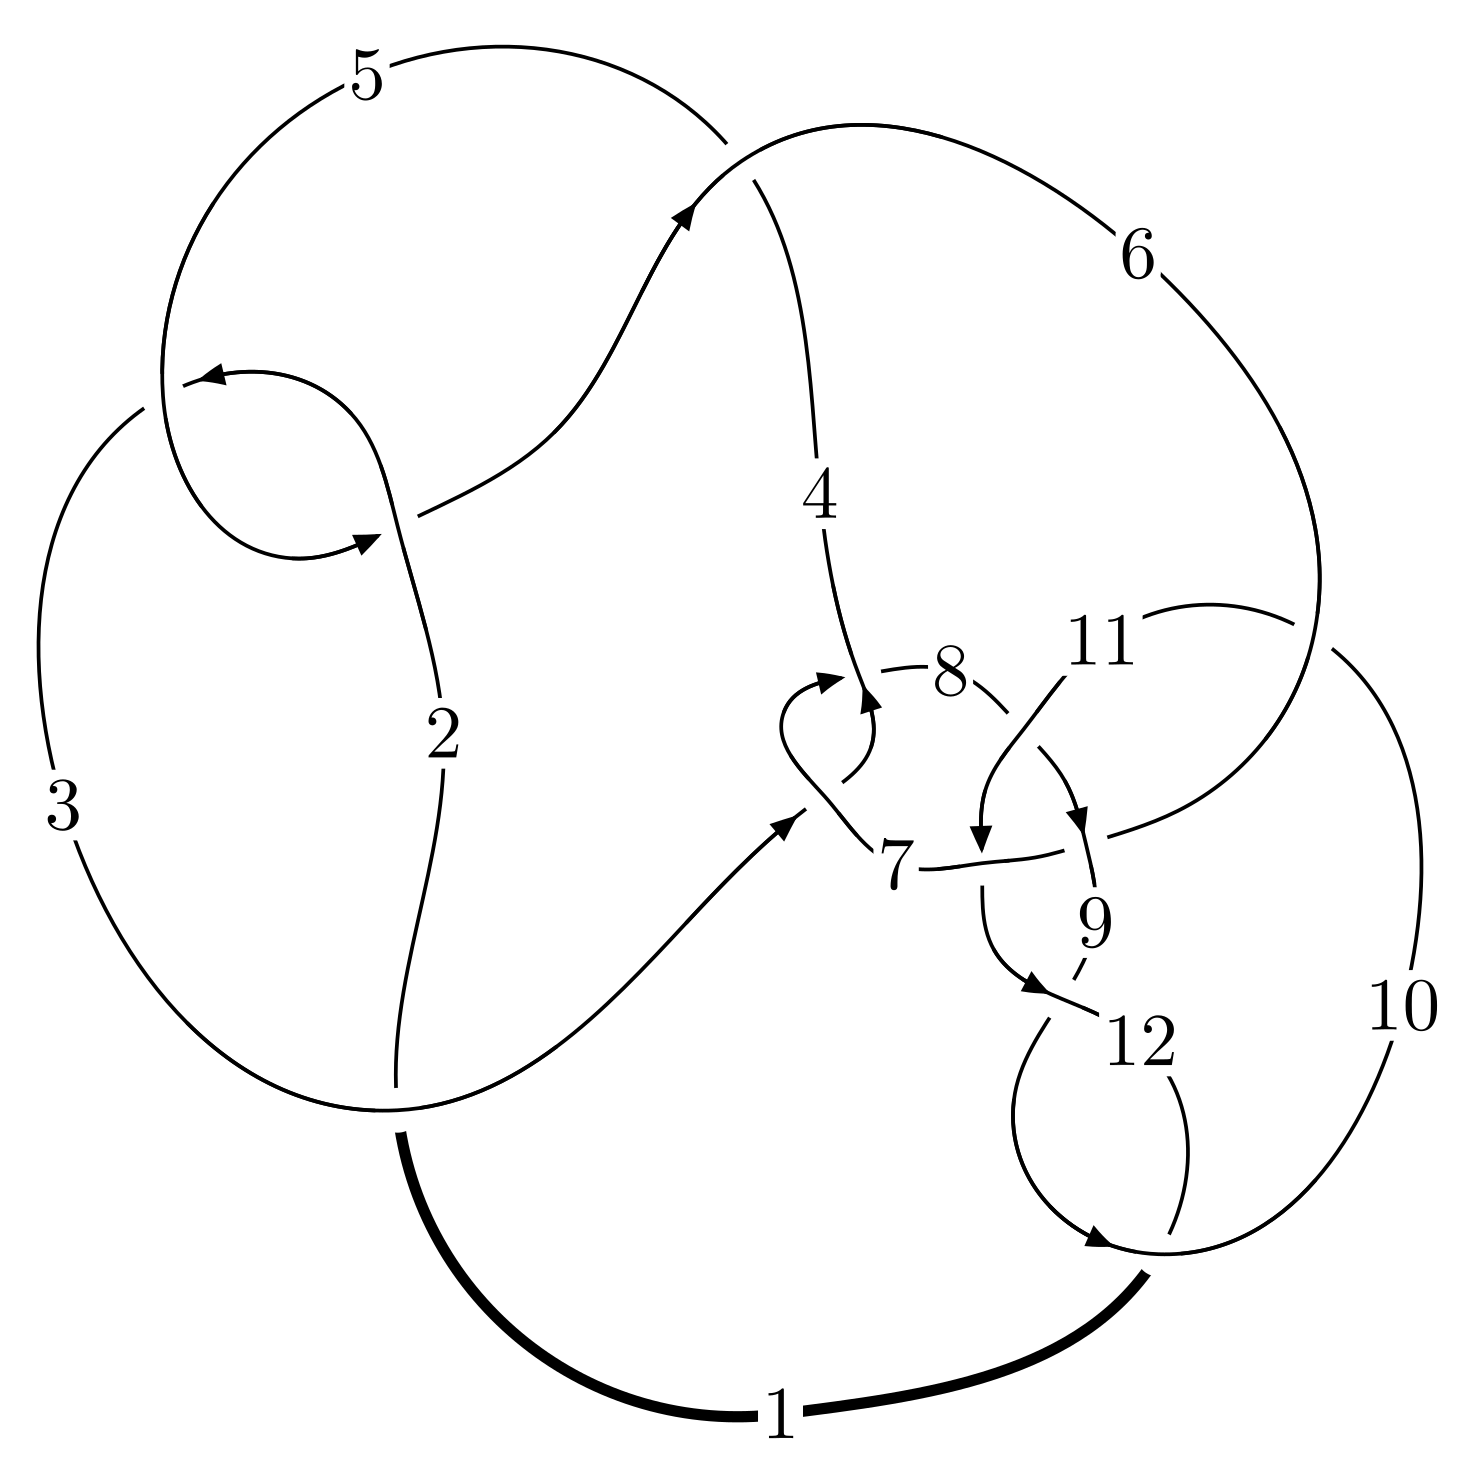
\includegraphics[width=112pt]{../../../GIT/diagram.site/Diagrams/png/2321_12n_0232.png}\\
\ \ \ A knot diagram\footnotemark}&
\allowdisplaybreaks
\textbf{Linearized knot diagam} \\
\cline{2-2}
 &
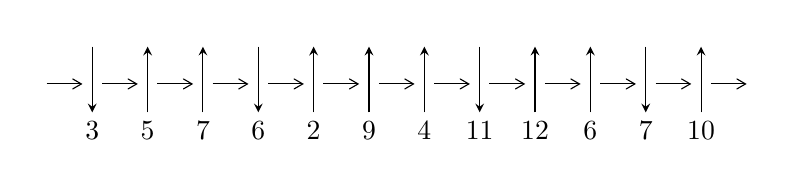
\begin{tikzpicture}[x=20pt, y=17pt]
	% nodes
	\node (C0) at (0, 0) {};
	\node (C1) at (1, 0) {};
	\node (C1U) at (1, +1) {};
	\node (C1D) at (1, -1) {3};

	\node (C2) at (2, 0) {};
	\node (C2U) at (2, +1) {};
	\node (C2D) at (2, -1) {5};

	\node (C3) at (3, 0) {};
	\node (C3U) at (3, +1) {};
	\node (C3D) at (3, -1) {7};

	\node (C4) at (4, 0) {};
	\node (C4U) at (4, +1) {};
	\node (C4D) at (4, -1) {6};

	\node (C5) at (5, 0) {};
	\node (C5U) at (5, +1) {};
	\node (C5D) at (5, -1) {2};

	\node (C6) at (6, 0) {};
	\node (C6U) at (6, +1) {};
	\node (C6D) at (6, -1) {9};

	\node (C7) at (7, 0) {};
	\node (C7U) at (7, +1) {};
	\node (C7D) at (7, -1) {4};

	\node (C8) at (8, 0) {};
	\node (C8U) at (8, +1) {};
	\node (C8D) at (8, -1) {11};

	\node (C9) at (9, 0) {};
	\node (C9U) at (9, +1) {};
	\node (C9D) at (9, -1) {12};

	\node (C10) at (10, 0) {};
	\node (C10U) at (10, +1) {};
	\node (C10D) at (10, -1) {6};

	\node (C11) at (11, 0) {};
	\node (C11U) at (11, +1) {};
	\node (C11D) at (11, -1) {7};

	\node (C12) at (12, 0) {};
	\node (C12U) at (12, +1) {};
	\node (C12D) at (12, -1) {10};
	\node (C13) at (13, 0) {};

	% arrows
	\draw[->,>={angle 60}]
	(C0) edge (C1) (C1) edge (C2) (C2) edge (C3) (C3) edge (C4) (C4) edge (C5) (C5) edge (C6) (C6) edge (C7) (C7) edge (C8) (C8) edge (C9) (C9) edge (C10) (C10) edge (C11) (C11) edge (C12) (C12) edge (C13) ;	\draw[->,>=stealth]
	(C1U) edge (C1D) (C2D) edge (C2U) (C3D) edge (C3U) (C4U) edge (C4D) (C5D) edge (C5U) (C6D) edge (C6U) (C7D) edge (C7U) (C8U) edge (C8D) (C9D) edge (C9U) (C10D) edge (C10U) (C11U) edge (C11D) (C12D) edge (C12U) ;
	\end{tikzpicture} \\
\hhline{~~} \\& 
\textbf{Solving Sequence} \\ \cline{2-2} 
 &
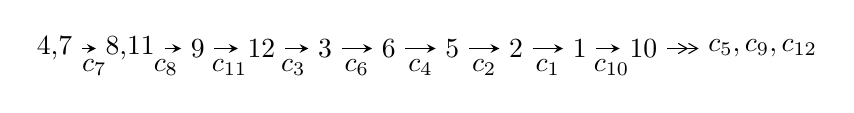
\begin{tikzpicture}[x=23pt, y=7pt]
	% node
	\node (A0) at (-1/8, 0) {4,7};
	\node (A1) at (17/16, 0) {8,11};
	\node (A2) at (17/8, 0) {9};
	\node (A3) at (25/8, 0) {12};
	\node (A4) at (33/8, 0) {3};
	\node (A5) at (41/8, 0) {6};
	\node (A6) at (49/8, 0) {5};
	\node (A7) at (57/8, 0) {2};
	\node (A8) at (65/8, 0) {1};
	\node (A9) at (73/8, 0) {10};
	\node (C1) at (1/2, -1) {$c_{7}$};
	\node (C2) at (13/8, -1) {$c_{8}$};
	\node (C3) at (21/8, -1) {$c_{11}$};
	\node (C4) at (29/8, -1) {$c_{3}$};
	\node (C5) at (37/8, -1) {$c_{6}$};
	\node (C6) at (45/8, -1) {$c_{4}$};
	\node (C7) at (53/8, -1) {$c_{2}$};
	\node (C8) at (61/8, -1) {$c_{1}$};
	\node (C9) at (69/8, -1) {$c_{10}$};
	\node (A10) at (11, 0) {$c_{5},c_{9},c_{12}$};

	% edge
	\draw[->,>=stealth]	
	(A0) edge (A1) (A1) edge (A2) (A2) edge (A3) (A3) edge (A4) (A4) edge (A5) (A5) edge (A6) (A6) edge (A7) (A7) edge (A8) (A8) edge (A9) ;
	\draw[->>,>={angle 60}]	
	(A9) edge (A10);
\end{tikzpicture} \\ 

\end{tabular} \\

\footnotetext{
The image of knot diagram is generated by the software ``\textbf{Draw programme}" developed by Andrew Bartholomew(\url{http://www.layer8.co.uk/maths/draw/index.htm\#Running-draw}), where we modified some parts for our purpose(\url{https://github.com/CATsTAILs/LinksPainter}).
}\phantom \\ \newline 
\centering \textbf{Ideals for irreducible components\footnotemark of $X_{\text{par}}$} 
 
\begin{align*}
I^u_{1}&=\langle 
-1.48632\times10^{99} u^{33}-5.79126\times10^{99} u^{32}+\cdots+9.25530\times10^{102} b-2.38605\times10^{103},\\
\phantom{I^u_{1}}&\phantom{= \langle  }-3.67965\times10^{100} u^{33}-2.13068\times10^{101} u^{32}+\cdots+3.70212\times10^{103} a-8.18316\times10^{104},\\
\phantom{I^u_{1}}&\phantom{= \langle  }u^{34}+2 u^{33}+\cdots-3072 u+1024\rangle \\
I^u_{2}&=\langle 
u^8-3 u^6- u^5+4 u^4+2 u^3- u^2+b-2 u-1,\;u^8+2 u^7-2 u^6-5 u^5+u^4+5 u^3+u^2+a,\\
\phantom{I^u_{2}}&\phantom{= \langle  }u^9+u^8-2 u^7-3 u^6+u^5+3 u^4+2 u^3- u-1\rangle \\
\\
I^v_{1}&=\langle 
a,\;1728 v^9-4936 v^8+9872 v^7+12908 v^6-24680 v^5-34552 v^4+91527 v^3+4936 v^2+3335 b-613,\\
\phantom{I^v_{1}}&\phantom{= \langle  }v^{10}-3 v^9+6 v^8+7 v^7-16 v^6-19 v^5+58 v^4-2 v^3-7 v^2- v+1\rangle \\
\end{align*}
\raggedright * 3 irreducible components of $\dim_{\mathbb{C}}=0$, with total 53 representations.\\
\footnotetext{All coefficients of polynomials are rational numbers. But the coefficients are sometimes approximated in decimal forms when there is not enough margin.}
\newpage
\renewcommand{\arraystretch}{1}
\centering \section*{I. $I^u_{1}= \langle -1.49\times10^{99} u^{33}-5.79\times10^{99} u^{32}+\cdots+9.26\times10^{102} b-2.39\times10^{103},\;-3.68\times10^{100} u^{33}-2.13\times10^{101} u^{32}+\cdots+3.70\times10^{103} a-8.18\times10^{104},\;u^{34}+2 u^{33}+\cdots-3072 u+1024 \rangle$}
\flushleft \textbf{(i) Arc colorings}\\
\begin{tabular}{m{7pt} m{180pt} m{7pt} m{180pt} }
\flushright $a_{4}=$&$\begin{pmatrix}0\\u\end{pmatrix}$ \\
\flushright $a_{7}=$&$\begin{pmatrix}1\\0\end{pmatrix}$ \\
\flushright $a_{8}=$&$\begin{pmatrix}1\\- u^2\end{pmatrix}$ \\
\flushright $a_{11}=$&$\begin{pmatrix}0.000993930 u^{33}+0.00575530 u^{32}+\cdots-34.8075 u+22.1040\\0.000160592 u^{33}+0.000625724 u^{32}+\cdots-5.64954 u+2.57803\end{pmatrix}$ \\
\flushright $a_{9}=$&$\begin{pmatrix}-0.00135334 u^{33}-0.00441762 u^{32}+\cdots+6.87137 u-7.96186\\0.000582441 u^{33}+0.00154725 u^{32}+\cdots+2.00787 u-0.0842617\end{pmatrix}$ \\
\flushright $a_{12}=$&$\begin{pmatrix}0.000833338 u^{33}+0.00512957 u^{32}+\cdots-29.1579 u+19.5259\\0.000160592 u^{33}+0.000625724 u^{32}+\cdots-5.64954 u+2.57803\end{pmatrix}$ \\
\flushright $a_{3}=$&$\begin{pmatrix}- u\\u\end{pmatrix}$ \\
\flushright $a_{6}=$&$\begin{pmatrix}0.00199895 u^{33}+0.00538241 u^{32}+\cdots-0.684374 u+3.58838\\-0.00147460 u^{33}-0.00388109 u^{32}+\cdots-4.51110 u+1.52261\end{pmatrix}$ \\
\flushright $a_{5}=$&$\begin{pmatrix}-0.000983560 u^{33}-0.00100646 u^{32}+\cdots-17.7146 u+4.94069\\-0.000685051 u^{33}-0.00177065 u^{32}+\cdots-1.78423 u+1.03576\end{pmatrix}$ \\
\flushright $a_{2}=$&$\begin{pmatrix}-0.000524358 u^{33}-0.00150131 u^{32}+\cdots+5.19547 u-5.11099\\-0.00147460 u^{33}-0.00388109 u^{32}+\cdots-4.51110 u+1.52261\end{pmatrix}$ \\
\flushright $a_{1}=$&$\begin{pmatrix}-0.000790332 u^{33}-0.00216412 u^{32}+\cdots+2.98921 u-3.69326\\-0.00120862 u^{33}-0.00321829 u^{32}+\cdots-2.30484 u+0.104878\end{pmatrix}$ \\
\flushright $a_{10}=$&$\begin{pmatrix}-0.000643181 u^{33}+0.000310006 u^{32}+\cdots-24.6133 u+14.9301\\0.000927418 u^{33}+0.00308742 u^{32}+\cdots-3.88840 u+1.37424\end{pmatrix}$\\&\end{tabular}
\flushleft \textbf{(ii) Obstruction class $= -1$}\\~\\
\flushleft \textbf{(iii) Cusp Shapes $= 0.0110768 u^{33}+0.0125415 u^{32}+\cdots+188.174 u-59.8533$}\\~\\
\newpage\renewcommand{\arraystretch}{1}
\flushleft \textbf{(iv) u-Polynomials at the component}\newline \\
\begin{tabular}{m{50pt}|m{274pt}}
Crossings & \hspace{64pt}u-Polynomials at each crossing \\
\hline $$\begin{aligned}c_{1},c_{4}\end{aligned}$$&$\begin{aligned}
&u^{34}+23 u^{33}+\cdots-148 u+1
\end{aligned}$\\
\hline $$\begin{aligned}c_{2},c_{5}\end{aligned}$$&$\begin{aligned}
&u^{34}+7 u^{33}+\cdots-74 u^2+1
\end{aligned}$\\
\hline $$\begin{aligned}c_{3},c_{7}\end{aligned}$$&$\begin{aligned}
&u^{34}+2 u^{33}+\cdots-3072 u+1024
\end{aligned}$\\
\hline $$\begin{aligned}c_{6}\end{aligned}$$&$\begin{aligned}
&u^{34}+4 u^{33}+\cdots-3 u-1
\end{aligned}$\\
\hline $$\begin{aligned}c_{8}\end{aligned}$$&$\begin{aligned}
&u^{34}-3 u^{33}+\cdots-5632 u+512
\end{aligned}$\\
\hline $$\begin{aligned}c_{9},c_{12}\end{aligned}$$&$\begin{aligned}
&u^{34}+12 u^{33}+\cdots-11 u-1
\end{aligned}$\\
\hline $$\begin{aligned}c_{10}\end{aligned}$$&$\begin{aligned}
&u^{34}-4 u^{33}+\cdots-666199 u+339173
\end{aligned}$\\
\hline $$\begin{aligned}c_{11}\end{aligned}$$&$\begin{aligned}
&u^{34}+2 u^{33}+\cdots-10595 u+25489
\end{aligned}$\\
\hline
\end{tabular}\\~\\
\newpage\renewcommand{\arraystretch}{1}
\flushleft \textbf{(v) Riley Polynomials at the component}\newline \\
\begin{tabular}{m{50pt}|m{274pt}}
Crossings & \hspace{64pt}Riley Polynomials at each crossing \\
\hline $$\begin{aligned}c_{1},c_{4}\end{aligned}$$&$\begin{aligned}
&y^{34}-17 y^{33}+\cdots-14096 y+1
\end{aligned}$\\
\hline $$\begin{aligned}c_{2},c_{5}\end{aligned}$$&$\begin{aligned}
&y^{34}+23 y^{33}+\cdots-148 y+1
\end{aligned}$\\
\hline $$\begin{aligned}c_{3},c_{7}\end{aligned}$$&$\begin{aligned}
&y^{34}+50 y^{33}+\cdots+1048576 y+1048576
\end{aligned}$\\
\hline $$\begin{aligned}c_{6}\end{aligned}$$&$\begin{aligned}
&y^{34}-4 y^{33}+\cdots-19 y+1
\end{aligned}$\\
\hline $$\begin{aligned}c_{8}\end{aligned}$$&$\begin{aligned}
&y^{34}-51 y^{33}+\cdots-3407872 y+262144
\end{aligned}$\\
\hline $$\begin{aligned}c_{9},c_{12}\end{aligned}$$&$\begin{aligned}
&y^{34}-4 y^{33}+\cdots+65 y+1
\end{aligned}$\\
\hline $$\begin{aligned}c_{10}\end{aligned}$$&$\begin{aligned}
&y^{34}+60 y^{33}+\cdots-783443850999 y+115038323929
\end{aligned}$\\
\hline $$\begin{aligned}c_{11}\end{aligned}$$&$\begin{aligned}
&y^{34}-36 y^{33}+\cdots+7287355609 y+649689121
\end{aligned}$\\
\hline
\end{tabular}\\~\\
\newpage\flushleft \textbf{(vi) Complex Volumes and Cusp Shapes}
$$\begin{array}{c|c|c}  
\text{Solutions to }I^u_{1}& \I (\text{vol} + \sqrt{-1}CS) & \text{Cusp shape}\\
 \hline 
\begin{aligned}
u &= \phantom{-}1.01886\phantom{ +0.000000I} \\
a &= \phantom{-}0.402417\phantom{ +0.000000I} \\
b &= -0.825508\phantom{ +0.000000I}\end{aligned}
 & \phantom{-}1.38631\phantom{ +0.000000I} & \phantom{-}7.11490\phantom{ +0.000000I} \\ \hline\begin{aligned}
u &= \phantom{-}0.946524 + 0.004818 I \\
a &= \phantom{-}0.0881160 - 0.0882313 I \\
b &= -0.622736 + 0.920702 I\end{aligned}
 & \phantom{-}6.54075 + 2.05806 I & \phantom{-}13.8961 - 2.8397 I \\ \hline\begin{aligned}
u &= \phantom{-}0.946524 - 0.004818 I \\
a &= \phantom{-}0.0881160 + 0.0882313 I \\
b &= -0.622736 - 0.920702 I\end{aligned}
 & \phantom{-}6.54075 - 2.05806 I & \phantom{-}13.8961 + 2.8397 I \\ \hline\begin{aligned}
u &= -0.764707 + 0.536808 I \\
a &= \phantom{-}0.0835054 + 0.0924226 I \\
b &= -0.236214 - 0.979802 I\end{aligned}
 & \phantom{-}6.07730 - 7.11588 I & \phantom{-}12.1179 + 9.6630 I \\ \hline\begin{aligned}
u &= -0.764707 - 0.536808 I \\
a &= \phantom{-}0.0835054 - 0.0924226 I \\
b &= -0.236214 + 0.979802 I\end{aligned}
 & \phantom{-}6.07730 + 7.11588 I & \phantom{-}12.1179 - 9.6630 I \\ \hline\begin{aligned}
u &= -0.305197 + 0.863434 I \\
a &= \phantom{-}1.356410 - 0.154788 I \\
b &= \phantom{-}0.691749 + 0.367275 I\end{aligned}
 & \phantom{-}0.62542 + 2.57137 I & \phantom{-}3.17282 - 2.86214 I \\ \hline\begin{aligned}
u &= -0.305197 - 0.863434 I \\
a &= \phantom{-}1.356410 + 0.154788 I \\
b &= \phantom{-}0.691749 - 0.367275 I\end{aligned}
 & \phantom{-}0.62542 - 2.57137 I & \phantom{-}3.17282 + 2.86214 I \\ \hline\begin{aligned}
u &= -0.642836 + 0.443818 I \\
a &= \phantom{-}0.488581 + 0.467682 I \\
b &= \phantom{-}0.115474 + 0.349761 I\end{aligned}
 & -1.59132 - 1.76956 I & -2.73476 + 4.21364 I \\ \hline\begin{aligned}
u &= -0.642836 - 0.443818 I \\
a &= \phantom{-}0.488581 - 0.467682 I \\
b &= \phantom{-}0.115474 - 0.349761 I\end{aligned}
 & -1.59132 + 1.76956 I & -2.73476 - 4.21364 I \\ \hline\begin{aligned}
u &= -0.732513 + 0.269955 I \\
a &= \phantom{-}2.27941 - 2.52971 I \\
b &= -0.05782 + 1.46259 I\end{aligned}
 & \phantom{-}0.72250 + 2.82980 I & \phantom{-}10.05148 - 3.22591 I\\
 \hline 
 \end{array}$$\newpage$$\begin{array}{c|c|c}  
\text{Solutions to }I^u_{1}& \I (\text{vol} + \sqrt{-1}CS) & \text{Cusp shape}\\
 \hline 
\begin{aligned}
u &= -0.732513 - 0.269955 I \\
a &= \phantom{-}2.27941 + 2.52971 I \\
b &= -0.05782 - 1.46259 I\end{aligned}
 & \phantom{-}0.72250 - 2.82980 I & \phantom{-}10.05148 + 3.22591 I \\ \hline\begin{aligned}
u &= \phantom{-}0.678106 + 0.349109 I \\
a &= \phantom{-}2.13499 + 2.18985 I \\
b &= -0.369797 - 0.819998 I\end{aligned}
 & \phantom{-}1.56878 + 0.34703 I & \phantom{-}8.40786 - 0.51532 I \\ \hline\begin{aligned}
u &= \phantom{-}0.678106 - 0.349109 I \\
a &= \phantom{-}2.13499 - 2.18985 I \\
b &= -0.369797 + 0.819998 I\end{aligned}
 & \phantom{-}1.56878 - 0.34703 I & \phantom{-}8.40786 + 0.51532 I \\ \hline\begin{aligned}
u &= \phantom{-}0.062735 + 0.467390 I \\
a &= \phantom{-}0.893723 + 0.003916 I \\
b &= \phantom{-}0.331665 - 0.940404 I\end{aligned}
 & \phantom{-}0.61291 + 1.48611 I & \phantom{-}4.79533 - 4.74523 I \\ \hline\begin{aligned}
u &= \phantom{-}0.062735 - 0.467390 I \\
a &= \phantom{-}0.893723 - 0.003916 I \\
b &= \phantom{-}0.331665 + 0.940404 I\end{aligned}
 & \phantom{-}0.61291 - 1.48611 I & \phantom{-}4.79533 + 4.74523 I \\ \hline\begin{aligned}
u &= \phantom{-}0.074045 + 0.443473 I \\
a &= \phantom{-}8.71021 + 1.02714 I \\
b &= \phantom{-}1.33192 - 0.57161 I\end{aligned}
 & \phantom{-}2.15188 + 2.20308 I & -18.1536 + 5.4483 I \\ \hline\begin{aligned}
u &= \phantom{-}0.074045 - 0.443473 I \\
a &= \phantom{-}8.71021 - 1.02714 I \\
b &= \phantom{-}1.33192 + 0.57161 I\end{aligned}
 & \phantom{-}2.15188 - 2.20308 I & -18.1536 - 5.4483 I \\ \hline\begin{aligned}
u &= \phantom{-}1.12191 + 1.21427 I \\
a &= \phantom{-}0.292658 - 0.148357 I \\
b &= \phantom{-}0.94260 + 1.15777 I\end{aligned}
 & -2.99715 - 2.34695 I & \phantom{-}4.00000 + 3.07511 I \\ \hline\begin{aligned}
u &= \phantom{-}1.12191 - 1.21427 I \\
a &= \phantom{-}0.292658 + 0.148357 I \\
b &= \phantom{-}0.94260 - 1.15777 I\end{aligned}
 & -2.99715 + 2.34695 I & \phantom{-}4.00000 - 3.07511 I \\ \hline\begin{aligned}
u &= \phantom{-}0.305756\phantom{ +0.000000I} \\
a &= \phantom{-}4.77767\phantom{ +0.000000I} \\
b &= -1.04203\phantom{ +0.000000I}\end{aligned}
 & \phantom{-}2.29528\phantom{ +0.000000I} & \phantom{-}1.25710\phantom{ +0.000000I}\\
 \hline 
 \end{array}$$\newpage$$\begin{array}{c|c|c}  
\text{Solutions to }I^u_{1}& \I (\text{vol} + \sqrt{-1}CS) & \text{Cusp shape}\\
 \hline 
\begin{aligned}
u &= -0.56509 + 2.04215 I \\
a &= -0.773555 + 0.263179 I \\
b &= -1.39864 - 0.29584 I\end{aligned}
 & -7.72558 - 0.90268 I & \phantom{-0.000000 } 0 \\ \hline\begin{aligned}
u &= -0.56509 - 2.04215 I \\
a &= -0.773555 - 0.263179 I \\
b &= -1.39864 + 0.29584 I\end{aligned}
 & -7.72558 + 0.90268 I & \phantom{-0.000000 } 0 \\ \hline\begin{aligned}
u &= \phantom{-}1.02869 + 1.89861 I \\
a &= -0.706865 - 0.350243 I \\
b &= -1.26804 + 0.74707 I\end{aligned}
 & -11.18750 + 7.23815 I & \phantom{-0.000000 } 0 \\ \hline\begin{aligned}
u &= \phantom{-}1.02869 - 1.89861 I \\
a &= -0.706865 + 0.350243 I \\
b &= -1.26804 - 0.74707 I\end{aligned}
 & -11.18750 - 7.23815 I & \phantom{-0.000000 } 0 \\ \hline\begin{aligned}
u &= -1.91642 + 1.10283 I \\
a &= \phantom{-}0.054061 + 0.259519 I \\
b &= -2.33781 + 0.73216 I\end{aligned}
 & -3.63061 - 2.77360 I & \phantom{-0.000000 } 0 \\ \hline\begin{aligned}
u &= -1.91642 - 1.10283 I \\
a &= \phantom{-}0.054061 - 0.259519 I \\
b &= -2.33781 - 0.73216 I\end{aligned}
 & -3.63061 + 2.77360 I & \phantom{-0.000000 } 0 \\ \hline\begin{aligned}
u &= -1.19908 + 1.98984 I \\
a &= \phantom{-}0.816613 - 0.366169 I \\
b &= \phantom{-}1.73482 + 1.78350 I\end{aligned}
 & -10.8926 - 14.7212 I & \phantom{-0.000000 } 0 \\ \hline\begin{aligned}
u &= -1.19908 - 1.98984 I \\
a &= \phantom{-}0.816613 + 0.366169 I \\
b &= \phantom{-}1.73482 - 1.78350 I\end{aligned}
 & -10.8926 + 14.7212 I & \phantom{-0.000000 } 0 \\ \hline\begin{aligned}
u &= \phantom{-}0.77518 + 2.27315 I \\
a &= \phantom{-}0.803096 + 0.162714 I \\
b &= \phantom{-}2.06341 - 1.43354 I\end{aligned}
 & -7.46169 + 8.00267 I & \phantom{-0.000000 } 0 \\ \hline\begin{aligned}
u &= \phantom{-}0.77518 - 2.27315 I \\
a &= \phantom{-}0.803096 - 0.162714 I \\
b &= \phantom{-}2.06341 + 1.43354 I\end{aligned}
 & -7.46169 - 8.00267 I & \phantom{-0.000000 } 0\\
 \hline 
 \end{array}$$\newpage$$\begin{array}{c|c|c}  
\text{Solutions to }I^u_{1}& \I (\text{vol} + \sqrt{-1}CS) & \text{Cusp shape}\\
 \hline 
\begin{aligned}
u &= -0.04194 + 2.58121 I \\
a &= -0.741302 - 0.045471 I \\
b &= -1.88206 - 0.20245 I\end{aligned}
 & -13.09350 - 4.80207 I & \phantom{-0.000000 } 0 \\ \hline\begin{aligned}
u &= -0.04194 - 2.58121 I \\
a &= -0.741302 + 0.045471 I \\
b &= -1.88206 + 0.20245 I\end{aligned}
 & -13.09350 + 4.80207 I & \phantom{-0.000000 } 0 \\ \hline\begin{aligned}
u &= -0.18171 + 2.97411 I \\
a &= \phantom{-}0.630299 + 0.012157 I \\
b &= \phantom{-}2.89525 + 1.03267 I\end{aligned}
 & -13.37580 - 1.94532 I & \phantom{-0.000000 } 0 \\ \hline\begin{aligned}
u &= -0.18171 - 2.97411 I \\
a &= \phantom{-}0.630299 - 0.012157 I \\
b &= \phantom{-}2.89525 - 1.03267 I\end{aligned}
 & -13.37580 + 1.94532 I & \phantom{-0.000000 } 0\\
 \hline 
 \end{array}$$\newpage\newpage\renewcommand{\arraystretch}{1}
\centering \section*{II. $I^u_{2}= \langle u^8-3 u^6- u^5+4 u^4+2 u^3- u^2+b-2 u-1,\;u^8+2 u^7-2 u^6-5 u^5+u^4+5 u^3+u^2+a,\;u^9+u^8-2 u^7-3 u^6+u^5+3 u^4+2 u^3- u-1 \rangle$}
\flushleft \textbf{(i) Arc colorings}\\
\begin{tabular}{m{7pt} m{180pt} m{7pt} m{180pt} }
\flushright $a_{4}=$&$\begin{pmatrix}0\\u\end{pmatrix}$ \\
\flushright $a_{7}=$&$\begin{pmatrix}1\\0\end{pmatrix}$ \\
\flushright $a_{8}=$&$\begin{pmatrix}1\\- u^2\end{pmatrix}$ \\
\flushright $a_{11}=$&$\begin{pmatrix}- u^8-2 u^7+2 u^6+5 u^5- u^4-5 u^3- u^2\\- u^8+3 u^6+u^5-4 u^4-2 u^3+u^2+2 u+1\end{pmatrix}$ \\
\flushright $a_{9}=$&$\begin{pmatrix}1\\- u^2\end{pmatrix}$ \\
\flushright $a_{12}=$&$\begin{pmatrix}-2 u^7- u^6+4 u^5+3 u^4-3 u^3-2 u^2-2 u-1\\- u^8+3 u^6+u^5-4 u^4-2 u^3+u^2+2 u+1\end{pmatrix}$ \\
\flushright $a_{3}=$&$\begin{pmatrix}- u\\u\end{pmatrix}$ \\
\flushright $a_{6}=$&$\begin{pmatrix}- u^2+1\\u^4\end{pmatrix}$ \\
\flushright $a_{5}=$&$\begin{pmatrix}- u^5+2 u^3- u\\u^7- u^5+u\end{pmatrix}$ \\
\flushright $a_{2}=$&$\begin{pmatrix}- u^4+u^2-1\\u^4\end{pmatrix}$ \\
\flushright $a_{1}=$&$\begin{pmatrix}-1\\u^2\end{pmatrix}$ \\
\flushright $a_{10}=$&$\begin{pmatrix}-2 u^7- u^6+4 u^5+3 u^4-3 u^3-2 u^2-2 u\\- u^8+3 u^6+u^5-4 u^4-2 u^3+2 u+1\end{pmatrix}$\\&\end{tabular}
\flushleft \textbf{(ii) Obstruction class $= 1$}\\~\\
\flushleft \textbf{(iii) Cusp Shapes $= 5 u^8+9 u^7-7 u^6-22 u^5-2 u^4+23 u^3+13 u^2+u+3$}\\~\\
\newpage\renewcommand{\arraystretch}{1}
\flushleft \textbf{(iv) u-Polynomials at the component}\newline \\
\begin{tabular}{m{50pt}|m{274pt}}
Crossings & \hspace{64pt}u-Polynomials at each crossing \\
\hline $$\begin{aligned}c_{1},c_{4}\end{aligned}$$&$\begin{aligned}
&u^9-3 u^8+8 u^7-13 u^6+17 u^5-17 u^4+12 u^3-6 u^2+u+1
\end{aligned}$\\
\hline $$\begin{aligned}c_{2}\end{aligned}$$&$\begin{aligned}
&u^9- u^8+2 u^7- u^6+3 u^5- u^4+2 u^3+u+1
\end{aligned}$\\
\hline $$\begin{aligned}c_{3}\end{aligned}$$&$\begin{aligned}
&u^9- u^8-2 u^7+3 u^6+u^5-3 u^4+2 u^3- u+1
\end{aligned}$\\
\hline $$\begin{aligned}c_{5}\end{aligned}$$&$\begin{aligned}
&u^9+u^8+2 u^7+u^6+3 u^5+u^4+2 u^3+u-1
\end{aligned}$\\
\hline $$\begin{aligned}c_{6}\end{aligned}$$&$\begin{aligned}
&u^9+5 u^8+12 u^7+15 u^6+9 u^5- u^4-4 u^3-2 u^2+u+1
\end{aligned}$\\
\hline $$\begin{aligned}c_{7}\end{aligned}$$&$\begin{aligned}
&u^9+u^8-2 u^7-3 u^6+u^5+3 u^4+2 u^3- u-1
\end{aligned}$\\
\hline $$\begin{aligned}c_{8}\end{aligned}$$&$\begin{aligned}
&u^9
\end{aligned}$\\
\hline $$\begin{aligned}c_{9}\end{aligned}$$&$\begin{aligned}
&(u+1)^9
\end{aligned}$\\
\hline $$\begin{aligned}c_{10},c_{11}\end{aligned}$$&$\begin{aligned}
&u^9+u^8-2 u^7-4 u^6- u^5+9 u^4+15 u^3+12 u^2+5 u+1
\end{aligned}$\\
\hline $$\begin{aligned}c_{12}\end{aligned}$$&$\begin{aligned}
&(u-1)^9
\end{aligned}$\\
\hline
\end{tabular}\\~\\
\newpage\renewcommand{\arraystretch}{1}
\flushleft \textbf{(v) Riley Polynomials at the component}\newline \\
\begin{tabular}{m{50pt}|m{274pt}}
Crossings & \hspace{64pt}Riley Polynomials at each crossing \\
\hline $$\begin{aligned}c_{1},c_{4}\end{aligned}$$&$\begin{aligned}
&y^9+7 y^8+20 y^7+25 y^6+5 y^5-15 y^4+22 y^2+13 y-1
\end{aligned}$\\
\hline $$\begin{aligned}c_{2},c_{5}\end{aligned}$$&$\begin{aligned}
&y^9+3 y^8+8 y^7+13 y^6+17 y^5+17 y^4+12 y^3+6 y^2+y-1
\end{aligned}$\\
\hline $$\begin{aligned}c_{3},c_{7}\end{aligned}$$&$\begin{aligned}
&y^9-5 y^8+12 y^7-15 y^6+9 y^5+y^4-4 y^3+2 y^2+y-1
\end{aligned}$\\
\hline $$\begin{aligned}c_{6}\end{aligned}$$&$\begin{aligned}
&y^9- y^8+12 y^7-7 y^6+37 y^5+y^4-10 y^2+5 y-1
\end{aligned}$\\
\hline $$\begin{aligned}c_{8}\end{aligned}$$&$\begin{aligned}
&y^9
\end{aligned}$\\
\hline $$\begin{aligned}c_{9},c_{12}\end{aligned}$$&$\begin{aligned}
&(y-1)^9
\end{aligned}$\\
\hline $$\begin{aligned}c_{10},c_{11}\end{aligned}$$&$\begin{aligned}
&y^9-5 y^8+10 y^7- y^5-37 y^4+7 y^3-12 y^2+y-1
\end{aligned}$\\
\hline
\end{tabular}\\~\\
\newpage\flushleft \textbf{(vi) Complex Volumes and Cusp Shapes}
$$\begin{array}{c|c|c}  
\text{Solutions to }I^u_{2}& \I (\text{vol} + \sqrt{-1}CS) & \text{Cusp shape}\\
 \hline 
\begin{aligned}
u &= -0.772920 + 0.510351 I \\
a &= \phantom{-}0.939568 - 0.981640 I \\
b &= \phantom{-}0.457852 + 1.072010 I\end{aligned}
 & -0.13850 - 2.09337 I & \phantom{-}3.38047 + 2.85927 I \\ \hline\begin{aligned}
u &= -0.772920 - 0.510351 I \\
a &= \phantom{-}0.939568 + 0.981640 I \\
b &= \phantom{-}0.457852 - 1.072010 I\end{aligned}
 & -0.13850 + 2.09337 I & \phantom{-}3.38047 - 2.85927 I \\ \hline\begin{aligned}
u &= \phantom{-}0.825933\phantom{ +0.000000I} \\
a &= -2.14893\phantom{ +0.000000I} \\
b &= \phantom{-}1.46592\phantom{ +0.000000I}\end{aligned}
 & \phantom{-}2.84338\phantom{ +0.000000I} & \phantom{-}17.4870\phantom{ +0.000000I} \\ \hline\begin{aligned}
u &= \phantom{-}1.173910 + 0.391555 I \\
a &= -0.119081 + 0.409451 I \\
b &= \phantom{-}0.522253 - 0.392004 I\end{aligned}
 & \phantom{-}6.01628 + 1.33617 I & \phantom{-}6.48878 + 2.15019 I \\ \hline\begin{aligned}
u &= \phantom{-}1.173910 - 0.391555 I \\
a &= -0.119081 - 0.409451 I \\
b &= \phantom{-}0.522253 + 0.392004 I\end{aligned}
 & \phantom{-}6.01628 - 1.33617 I & \phantom{-}6.48878 - 2.15019 I \\ \hline\begin{aligned}
u &= -0.141484 + 0.739668 I \\
a &= -2.26219 + 2.13290 I \\
b &= -1.63880 + 0.65075 I\end{aligned}
 & \phantom{-}2.26187 + 2.45442 I & \phantom{-}6.9022 - 12.4598 I \\ \hline\begin{aligned}
u &= -0.141484 - 0.739668 I \\
a &= -2.26219 - 2.13290 I \\
b &= -1.63880 - 0.65075 I\end{aligned}
 & \phantom{-}2.26187 - 2.45442 I & \phantom{-}6.9022 + 12.4598 I \\ \hline\begin{aligned}
u &= -1.172470 + 0.500383 I \\
a &= \phantom{-}0.016164 - 0.378317 I \\
b &= \phantom{-}0.425734 + 0.444312 I\end{aligned}
 & \phantom{-}5.24306 - 7.08493 I & \phantom{-}2.48514 + 6.49599 I \\ \hline\begin{aligned}
u &= -1.172470 - 0.500383 I \\
a &= \phantom{-}0.016164 + 0.378317 I \\
b &= \phantom{-}0.425734 - 0.444312 I\end{aligned}
 & \phantom{-}5.24306 + 7.08493 I & \phantom{-}2.48514 - 6.49599 I\\
 \hline 
 \end{array}$$\newpage\newpage\renewcommand{\arraystretch}{1}
\centering \section*{III. $I^v_{1}= \langle a,\;1728 v^9-4936 v^8+\cdots+3335 b-613,\;v^{10}-3 v^9+\cdots- v+1 \rangle$}
\flushleft \textbf{(i) Arc colorings}\\
\begin{tabular}{m{7pt} m{180pt} m{7pt} m{180pt} }
\flushright $a_{4}=$&$\begin{pmatrix}v\\0\end{pmatrix}$ \\
\flushright $a_{7}=$&$\begin{pmatrix}1\\0\end{pmatrix}$ \\
\flushright $a_{8}=$&$\begin{pmatrix}1\\0\end{pmatrix}$ \\
\flushright $a_{11}=$&$\begin{pmatrix}0\\-0.518141 v^{9}+1.48006 v^{8}+\cdots-1.48006 v^{2}+0.183808\end{pmatrix}$ \\
\flushright $a_{9}=$&$\begin{pmatrix}1\\0.462969 v^{9}-1.33373 v^{8}+\cdots+1.33373 v^{2}-1.81379\end{pmatrix}$ \\
\flushright $a_{12}=$&$\begin{pmatrix}0.518141 v^{9}-1.48006 v^{8}+\cdots+1.48006 v^{2}-0.183808\\-0.518141 v^{9}+1.48006 v^{8}+\cdots-1.48006 v^{2}+0.183808\end{pmatrix}$ \\
\flushright $a_{3}=$&$\begin{pmatrix}v\\0\end{pmatrix}$ \\
\flushright $a_{6}=$&$\begin{pmatrix}0.462969 v^{9}-1.33373 v^{8}+\cdots+1.33373 v^{2}-0.813793\\-1.14783 v^{9}+3.29565 v^{8}+\cdots-3.29565 v^{2}+1.75652\end{pmatrix}$ \\
\flushright $a_{5}=$&$\begin{pmatrix}0.0740630 v^{9}-0.148126 v^{8}+\cdots+3.77811 v-0.424888\\-0.147826 v^{9}+0.295652 v^{8}+\cdots-7 v+0.756522\end{pmatrix}$ \\
\flushright $a_{2}=$&$\begin{pmatrix}-0.610795 v^{9}+1.75982 v^{8}+\cdots+v+0.961619\\1.14783 v^{9}-3.29565 v^{8}+\cdots+3.29565 v^{2}-1.75652\end{pmatrix}$ \\
\flushright $a_{1}=$&$\begin{pmatrix}-0.462969 v^{9}+1.33373 v^{8}+\cdots-1.33373 v^{2}+0.813793\\1.14783 v^{9}-3.29565 v^{8}+\cdots+3.29565 v^{2}-1.75652\end{pmatrix}$ \\
\flushright $a_{10}=$&$\begin{pmatrix}-0.684858 v^{9}+1.96192 v^{8}+\cdots-1.96192 v^{2}+0.942729\\1.14783 v^{9}-3.29565 v^{8}+\cdots+3.29565 v^{2}-1.75652\end{pmatrix}$\\&\end{tabular}
\flushleft \textbf{(ii) Obstruction class $= 1$}\\~\\
\flushleft \textbf{(iii) Cusp Shapes $= \frac{1259}{667} v^9-\frac{146}{29} v^8+\frac{6397}{667} v^7+\frac{11075}{667} v^6-\frac{16703}{667} v^5-\frac{29857}{667} v^4+\frac{2799}{29} v^3+\frac{18061}{667} v^2-\frac{151}{23} v+\frac{990}{667}$}\\~\\
\newpage\renewcommand{\arraystretch}{1}
\flushleft \textbf{(iv) u-Polynomials at the component}\newline \\
\begin{tabular}{m{50pt}|m{274pt}}
Crossings & \hspace{64pt}u-Polynomials at each crossing \\
\hline $$\begin{aligned}c_{1},c_{4},c_{5}\end{aligned}$$&$\begin{aligned}
&(u^2- u+1)^5
\end{aligned}$\\
\hline $$\begin{aligned}c_{2}\end{aligned}$$&$\begin{aligned}
&(u^2+u+1)^5
\end{aligned}$\\
\hline $$\begin{aligned}c_{3},c_{7}\end{aligned}$$&$\begin{aligned}
&u^{10}
\end{aligned}$\\
\hline $$\begin{aligned}c_{6}\end{aligned}$$&$\begin{aligned}
&(u^5+3 u^4+4 u^3+u^2- u-1)^2
\end{aligned}$\\
\hline $$\begin{aligned}c_{8}\end{aligned}$$&$\begin{aligned}
&(u^5+u^4+2 u^3+u^2+u+1)^2
\end{aligned}$\\
\hline $$\begin{aligned}c_{9}\end{aligned}$$&$\begin{aligned}
&(u^5- u^4-2 u^3+u^2+u+1)^2
\end{aligned}$\\
\hline $$\begin{aligned}c_{10},c_{12}\end{aligned}$$&$\begin{aligned}
&(u^5+u^4-2 u^3- u^2+u-1)^2
\end{aligned}$\\
\hline $$\begin{aligned}c_{11}\end{aligned}$$&$\begin{aligned}
&(u^5- u^4+2 u^3- u^2+u-1)^2
\end{aligned}$\\
\hline
\end{tabular}\\~\\
\newpage\renewcommand{\arraystretch}{1}
\flushleft \textbf{(v) Riley Polynomials at the component}\newline \\
\begin{tabular}{m{50pt}|m{274pt}}
Crossings & \hspace{64pt}Riley Polynomials at each crossing \\
\hline $$\begin{aligned}c_{1},c_{2},c_{4}\\c_{5}\end{aligned}$$&$\begin{aligned}
&(y^2+y+1)^5
\end{aligned}$\\
\hline $$\begin{aligned}c_{3},c_{7}\end{aligned}$$&$\begin{aligned}
&y^{10}
\end{aligned}$\\
\hline $$\begin{aligned}c_{6}\end{aligned}$$&$\begin{aligned}
&(y^5- y^4+8 y^3-3 y^2+3 y-1)^2
\end{aligned}$\\
\hline $$\begin{aligned}c_{8},c_{11}\end{aligned}$$&$\begin{aligned}
&(y^5+3 y^4+4 y^3+y^2- y-1)^2
\end{aligned}$\\
\hline $$\begin{aligned}c_{9},c_{10},c_{12}\end{aligned}$$&$\begin{aligned}
&(y^5-5 y^4+8 y^3-3 y^2- y-1)^2
\end{aligned}$\\
\hline
\end{tabular}\\~\\
\newpage\flushleft \textbf{(vi) Complex Volumes and Cusp Shapes}
$$\begin{array}{c|c|c}  
\text{Solutions to }I^v_{1}& \I (\text{vol} + \sqrt{-1}CS) & \text{Cusp shape}\\
 \hline 
\begin{aligned}
v &= \phantom{-}1.38814 + 0.78973 I \\
a &= \phantom{-0.000000 } 0 \\
b &= \phantom{-}0.339110 + 0.822375 I\end{aligned}
 & \phantom{-}0.329100 + 0.499304 I & \phantom{-}3.01153 - 0.88894 I \\ \hline\begin{aligned}
v &= \phantom{-}1.38814 - 0.78973 I \\
a &= \phantom{-0.000000 } 0 \\
b &= \phantom{-}0.339110 - 0.822375 I\end{aligned}
 & \phantom{-}0.329100 - 0.499304 I & \phantom{-}3.01153 + 0.88894 I \\ \hline\begin{aligned}
v &= -1.37799 + 0.80730 I \\
a &= \phantom{-0.000000 } 0 \\
b &= \phantom{-}0.339110 + 0.822375 I\end{aligned}
 & \phantom{-}0.32910 - 3.56046 I & \phantom{-}3.07628 + 9.77765 I \\ \hline\begin{aligned}
v &= -1.37799 - 0.80730 I \\
a &= \phantom{-0.000000 } 0 \\
b &= \phantom{-}0.339110 - 0.822375 I\end{aligned}
 & \phantom{-}0.32910 + 3.56046 I & \phantom{-}3.07628 - 9.77765 I \\ \hline\begin{aligned}
v &= -0.294694 + 0.220725 I \\
a &= \phantom{-0.000000 } 0 \\
b &= -0.455697 - 1.200150 I\end{aligned}
 & \phantom{-}5.87256 - 6.43072 I & \phantom{-}6.63163 + 0.01393 I \\ \hline\begin{aligned}
v &= -0.294694 - 0.220725 I \\
a &= \phantom{-0.000000 } 0 \\
b &= -0.455697 + 1.200150 I\end{aligned}
 & \phantom{-}5.87256 + 6.43072 I & \phantom{-}6.63163 - 0.01393 I \\ \hline\begin{aligned}
v &= \phantom{-}0.338500 + 0.144851 I \\
a &= \phantom{-0.000000 } 0 \\
b &= -0.455697 - 1.200150 I\end{aligned}
 & \phantom{-}5.87256 - 2.37095 I & \phantom{-}3.55752 + 5.27247 I \\ \hline\begin{aligned}
v &= \phantom{-}0.338500 - 0.144851 I \\
a &= \phantom{-0.000000 } 0 \\
b &= -0.455697 + 1.200150 I\end{aligned}
 & \phantom{-}5.87256 + 2.37095 I & \phantom{-}3.55752 - 5.27247 I \\ \hline\begin{aligned}
v &= \phantom{-}1.44605 + 2.50463 I \\
a &= \phantom{-0.000000 } 0 \\
b &= -0.766826\phantom{ +0.000000I}\end{aligned}
 & \phantom{-}2.40108 - 2.02988 I & \phantom{-}9.72304 - 3.67600 I \\ \hline\begin{aligned}
v &= \phantom{-}1.44605 - 2.50463 I \\
a &= \phantom{-0.000000 } 0 \\
b &= -0.766826\phantom{ +0.000000I}\end{aligned}
 & \phantom{-}2.40108 + 2.02988 I & \phantom{-}9.72304 + 3.67600 I\\
 \hline 
 \end{array}$$\newpage
\newpage\renewcommand{\arraystretch}{1}
\centering \section*{ IV. u-Polynomials}
\begin{tabular}{m{50pt}|m{274pt}}
Crossings & \hspace{64pt}u-Polynomials at each crossing \\
\hline $$\begin{aligned}c_{1},c_{4}\end{aligned}$$&$\begin{aligned}
&(u^2- u+1)^5\\
&\cdot(u^9-3 u^8+8 u^7-13 u^6+17 u^5-17 u^4+12 u^3-6 u^2+u+1)\\
&\cdot(u^{34}+23 u^{33}+\cdots-148 u+1)
\end{aligned}$\\
\hline $$\begin{aligned}c_{2}\end{aligned}$$&$\begin{aligned}
&(u^2+u+1)^5(u^9- u^8+2 u^7- u^6+3 u^5- u^4+2 u^3+u+1)\\
&\cdot(u^{34}+7 u^{33}+\cdots-74 u^2+1)
\end{aligned}$\\
\hline $$\begin{aligned}c_{3}\end{aligned}$$&$\begin{aligned}
&u^{10}(u^9- u^8-2 u^7+3 u^6+u^5-3 u^4+2 u^3- u+1)\\
&\cdot(u^{34}+2 u^{33}+\cdots-3072 u+1024)
\end{aligned}$\\
\hline $$\begin{aligned}c_{5}\end{aligned}$$&$\begin{aligned}
&(u^2- u+1)^5(u^9+u^8+2 u^7+u^6+3 u^5+u^4+2 u^3+u-1)\\
&\cdot(u^{34}+7 u^{33}+\cdots-74 u^2+1)
\end{aligned}$\\
\hline $$\begin{aligned}c_{6}\end{aligned}$$&$\begin{aligned}
&(u^5+3 u^4+4 u^3+u^2- u-1)^2\\
&\cdot(u^9+5 u^8+12 u^7+15 u^6+9 u^5- u^4-4 u^3-2 u^2+u+1)\\
&\cdot(u^{34}+4 u^{33}+\cdots-3 u-1)
\end{aligned}$\\
\hline $$\begin{aligned}c_{7}\end{aligned}$$&$\begin{aligned}
&u^{10}(u^9+u^8-2 u^7-3 u^6+u^5+3 u^4+2 u^3- u-1)\\
&\cdot(u^{34}+2 u^{33}+\cdots-3072 u+1024)
\end{aligned}$\\
\hline $$\begin{aligned}c_{8}\end{aligned}$$&$\begin{aligned}
&u^9(u^5+u^4+\cdots+u+1)^{2}(u^{34}-3 u^{33}+\cdots-5632 u+512)
\end{aligned}$\\
\hline $$\begin{aligned}c_{9}\end{aligned}$$&$\begin{aligned}
&((u+1)^9)(u^5- u^4+\cdots+u+1)^{2}(u^{34}+12 u^{33}+\cdots-11 u-1)
\end{aligned}$\\
\hline $$\begin{aligned}c_{10}\end{aligned}$$&$\begin{aligned}
&(u^5+u^4-2 u^3- u^2+u-1)^2\\
&\cdot(u^9+u^8-2 u^7-4 u^6- u^5+9 u^4+15 u^3+12 u^2+5 u+1)\\
&\cdot(u^{34}-4 u^{33}+\cdots-666199 u+339173)
\end{aligned}$\\
\hline $$\begin{aligned}c_{11}\end{aligned}$$&$\begin{aligned}
&(u^5- u^4+2 u^3- u^2+u-1)^2\\
&\cdot(u^9+u^8-2 u^7-4 u^6- u^5+9 u^4+15 u^3+12 u^2+5 u+1)\\
&\cdot(u^{34}+2 u^{33}+\cdots-10595 u+25489)
\end{aligned}$\\
\hline $$\begin{aligned}c_{12}\end{aligned}$$&$\begin{aligned}
&((u-1)^9)(u^5+u^4+\cdots+u-1)^{2}(u^{34}+12 u^{33}+\cdots-11 u-1)
\end{aligned}$\\
\hline
\end{tabular}\newpage\renewcommand{\arraystretch}{1}
\centering \section*{ V. Riley Polynomials}
\begin{tabular}{m{50pt}|m{274pt}}
Crossings & \hspace{64pt}Riley Polynomials at each crossing \\
\hline $$\begin{aligned}c_{1},c_{4}\end{aligned}$$&$\begin{aligned}
&((y^2+y+1)^5)(y^9+7 y^8+\cdots+13 y-1)\\
&\cdot(y^{34}-17 y^{33}+\cdots-14096 y+1)
\end{aligned}$\\
\hline $$\begin{aligned}c_{2},c_{5}\end{aligned}$$&$\begin{aligned}
&(y^2+y+1)^5\\
&\cdot(y^9+3 y^8+8 y^7+13 y^6+17 y^5+17 y^4+12 y^3+6 y^2+y-1)\\
&\cdot(y^{34}+23 y^{33}+\cdots-148 y+1)
\end{aligned}$\\
\hline $$\begin{aligned}c_{3},c_{7}\end{aligned}$$&$\begin{aligned}
&y^{10}(y^9-5 y^8+12 y^7-15 y^6+9 y^5+y^4-4 y^3+2 y^2+y-1)\\
&\cdot(y^{34}+50 y^{33}+\cdots+1048576 y+1048576)
\end{aligned}$\\
\hline $$\begin{aligned}c_{6}\end{aligned}$$&$\begin{aligned}
&(y^5- y^4+8 y^3-3 y^2+3 y-1)^2\\
&\cdot(y^9- y^8+12 y^7-7 y^6+37 y^5+y^4-10 y^2+5 y-1)\\
&\cdot(y^{34}-4 y^{33}+\cdots-19 y+1)
\end{aligned}$\\
\hline $$\begin{aligned}c_{8}\end{aligned}$$&$\begin{aligned}
&y^9(y^5+3 y^4+4 y^3+y^2- y-1)^2\\
&\cdot(y^{34}-51 y^{33}+\cdots-3407872 y+262144)
\end{aligned}$\\
\hline $$\begin{aligned}c_{9},c_{12}\end{aligned}$$&$\begin{aligned}
&((y-1)^9)(y^5-5 y^4+\cdots- y-1)^{2}(y^{34}-4 y^{33}+\cdots+65 y+1)
\end{aligned}$\\
\hline $$\begin{aligned}c_{10}\end{aligned}$$&$\begin{aligned}
&(y^5-5 y^4+8 y^3-3 y^2- y-1)^2\\
&\cdot(y^9-5 y^8+10 y^7- y^5-37 y^4+7 y^3-12 y^2+y-1)\\
&\cdot(y^{34}+60 y^{33}+\cdots-783443850999 y+115038323929)
\end{aligned}$\\
\hline $$\begin{aligned}c_{11}\end{aligned}$$&$\begin{aligned}
&(y^5+3 y^4+4 y^3+y^2- y-1)^2\\
&\cdot(y^9-5 y^8+10 y^7- y^5-37 y^4+7 y^3-12 y^2+y-1)\\
&\cdot(y^{34}-36 y^{33}+\cdots+7287355609 y+649689121)
\end{aligned}$\\
\hline
\end{tabular}
\vskip 2pc
\end{document}